


%%%%%%%%%%%%%%%%%%%%%%%%%%%%%%%%%%%%%%%%%%%%%%%%%%%%%%%%%%%%%%%%%%%%%%%%%%%%%%%
%%%%%%%%%%%%%%%%%%%%%%%%%%%%%%%%%%%%%%%%%%%%%%%%%%%%%%%%%%%%%%%%%%%%%%%%%%%%%%%
% APPENDIX
%%%%%%%%%%%%%%%%%%%%%%%%%%%%%%%%%%%%%%%%%%%%%%%%%%%%%%%%%%%%%%%%%%%%%%%%%%%%%%%
%%%%%%%%%%%%%%%%%%%%%%%%%%%%%%%%%%%%%%%%%%%%%%%%%%%%%%%%%%%%%%%%%%%%%%%%%%%%%%%



\section{Proofs}
\label{appendix:proofs}
Denote by $\msg(s)\triangleq \{ (t,s(t)): \eqsp t\in \msi \} $ the graph of a time series $s: \msi \to \Rset^d$ and $ \phi.\msg(s)\triangleq\{ \phi(t,s(t)): \eqsp t\in \msi\} $ the action of  $\phi\in \mcd(\Rset^{d+1}) $ on $\msg(s)$.
\begin{theorem}
    \label{theorem:representation_proof}
Let $s:  \msj \to \Rset^d  $ and $\mathbf{s}_0: \msi\to \Rset^d $ be two continuously differentiable time seriess with $\msi,\msj$ two intervals of $\Rset$.
 There exist $f\in \rmC^1(\Rset^{d+1},\Rset^d)$ and $\gamma\in  \mcd(\Rset) $ such that $\gamma(\msi)=\msj $ and $\Phi_f\in \mcd(\Rset^{d+1})$,
 \begin{equation}% TO add more detail on functionnal space
    \msg(s)= \Pi_{\gamma,f}.\msg(\mathbf{s}_0),\eqsp \Pi_{\gamma,f}=\Psi_\gamma\circ\Phi_f.
 \end{equation}
 Moreover, for any $\bar{f}\in \rmC^1(\Rset^{d+1},\Rset^d)$ and $\bar{\gamma}\in  \mcd(\Rset) $, there exists a continously differentiable time series $\bar{s}$ such that 
 $\msg(\bar{s})= \Pi_{\bar{\gamma},\bar{f}}.\msg(\mathbf{s}_0)$
\end{theorem}
%\sam{preuve todo, classement des variétés à bord, donne un homeomorphisme sur la restriction}
\begin{proof}
  Let $s:  \msj \to \Rset^d  $ and $\mathbf{s}_0: \msi\to \Rset^d $ be two continuously differentiable time seriess with $\msi=(a,b),\msj=(\alpha,\beta)$ two intervals of $\Rset$.
  By setting $\gamma: t\in \Rset \mapsto (\beta-\alpha)(t-a)/(b-a)+\alpha\in \Rset $, we have $ \gamma(\msi)=\msj$ and $\gamma \in \mcd(\Rset) $.
   By defining $f:(t,x)\in\Rset^{d+1}\mapsto x-\mathbf{s}_0(t)+s\circ \gamma(t) $, the map $\Phi_f\in \mcd(\Rset^{d+1})$,
    indeed, its inverse is $\Phi_f^{-1}:(t,x)\in\Rset^{d+1}\mapsto (t,x+\mathbf{s}_0(t)-s(t)) $ and is continuously differentiable.
     Moreover, we have $\Pi_{\gamma,f}.\msg(\mathbf{s}_0)=\{(\gamma(t),s\circ \gamma(t)):\eqsp t\in\msi \}=\msg(s) $.

    

    Let $\bar{f}\in \rmC^0(\Rset^{d+1},\Rset^d)$, $\bar{\gamma}\in  \mcd(\Rset) $ and $\mathbf{s}_0\in \rmC^0(\msi,\Rset^d)$ with $\msi$ an interval of $\Rset$.
    We have :
    \begin{align}
      \Pi_{\gamma,f}.\msg(\mathbf{s}_0)&=\{(\gamma(t),f(t,\mathbf{s}_0(t))),\eqsp t\in \msi \} \\
      &\label{eq:proof1_last_eq}=\{(t,f\left(\gamma^{-1}(t),\mathbf{s}_0(\gamma^{-1}(t))\right),\eqsp t\in \gamma(\msi) \} \eqsp .
    \end{align}
    By defining $\bar{s}:t\in \gamma(\msi)\to f\left(\gamma^{-1}(t),\mathbf{s}_0(\gamma^{-1}(t))\right) $, we have $\bar{s}\in \rmC^0(\gamma(\msi), \Rset^d) $ by composition of continuous functions
    and $ \msg(\bar{s})= \Pi_{\gamma,f}.\msg(\mathbf{s}_0)$ by \eqref{eq:proof1_last_eq}, which concludes the proof.
\end{proof}
\begin{lemma}
  If we denote by $\msv$ the RKHS associated with the kernel $K_{\msg}$, then for any vector field $v$ generated by \eqref{eq:integration} with $v_0$ satisfying \eqref{eq:def_v0},
   there exist $\gamma \in \msd(\Rset) $ and $f\in \rmC^1(\Rset^{d+1},\Rset^d)$ such that $\phi^v=\Psi_\gamma\circ\Phi_f $.
\end{lemma}
\begin{proof}
  Let $v$ be a vector field generated by \eqref{eq:integration} with $v_0$ satisfying \eqref{eq:def_v0}.
 We remark that the first coordinate of the velocity field $v_\tau$ denoted by $v_\tau^{\text{time}}$ only depends on the time variable $t$ for any $\tau\in[0,1]$.
 Thus, when computing the first coordinate of the deformation $\phi^v$, denoted by $\gamma$, we integrate \eqref{eq:LDDMM_dynamic} with $v_\tau$ replaced by $v_\tau^{\text{time}}$,
  thus $\gamma$ is independant of the variable $x$. Moreover, $\gamma\in \mcd(\Rset)$ since a Gaussian kernel induced an Hilbert space $\msv$ satisfying $|f|_V\leq |f|_\infty+ |\dd f|_\infty  $ for any $f\in \msv$ by \citep[Theorem 9]{glaunes2005transport}.
  For the same reason, we have $\phi^v\in \mcd(\Rset^{d+1})$, and thus its last coordinates denoted by $f$ belongs to $\rmC^1(\Rset^{d+1},\Rset^d)$, and by construction $\phi^v=\Psi_\gamma\circ\Phi_f $.
\end{proof}




\section{Oriented varifold}

\label{appendix:varifold}
In this section, we introduce the \textit{oriented varifold} associated with curves.
For further readings on curves and surfaces representation as varifolds, readers can refer to \cite{kaltenmark2017general,charon2013varifold}. 
We associate to $\gamma\in \rmC^1((a,b),\Rset^{d+1})$ an \textit{oriented varifold} $\mu_\gamma$, i.e. a distribution on the space $\Rset^{d+1}\times \mathbb{S}^{d}$ defined as follows, for any smooth test function $\omega :\Rset^{d+1}\times \mathbb{S}^{d}\to \Rset  $,
\begin{equation}
  \mathbb{E}_{Y\sim \mu_\gamma}\left[\omega(Y)\right]=\mu_\gamma(\omega)=\int_a^b \omega\left(\gamma(t),\frac{\dot{\gamma}(t)}{|\dot{\gamma}(t)|}\right)|\dot{\gamma}(t)|\dd t \eqsp .
\end{equation}
Denoting by $\msw$ the space of smooth test function, we have that $\mu_\gamma $ belongs to its dual $\msw^*$.
 Thus, a distance on $\msw^*$ is sufficient to set a distance on oriented varifolds associated to curve and thus on $\rmC^1((a,b),\Rset^{d+1})$ by the identification $\gamma\to \mu_\gamma $.
Remark that in (TS-LDDMM), $\gamma$ should be the parametrization of a time series' graph $\msg(s)$, i.e. $\gamma: t\in \msi \to (t,s(t))\in\Rset^{d+1} $ denoting by $s:\msi \to \Rset^d$ the time series.
However, in practice, we work with discrete objects.
 That is why, we set $W$ as an RKHS to use its representation theorem.
 More specifically \citep[Proposition 2 \& 4]{kaltenmark2017general} encourages us to consider a kernel $k:(\Rset^{d+1} \times \mathbb{S}^d)^2\to \Rset$ such that there exist two positive and continuously differentiable kernels $k_{\pos}$ and $k_{\dir}$, 
 such that for any $(x,\overrightarrow{u}),(y,\overrightarrow{v}) \in (\Rset^{d+1} \times \mathbb{S}^d)^2$
 \begin{equation}
     k((x,\overrightarrow{u}),(y,\overrightarrow{v})) = k_{\pos}(x,y)k_{\dir}(\overrightarrow{u},\overrightarrow{v}) \eqsp,
   \end{equation}
 with moreover $k_\dir>0$ and $ k_\pos$ which admits an RKHS $\msw_\pos$ dense in the space of continous function on $\Rset^{d+1}$ vanishing at infinite \cite{carmeli2010vector}.

Given such a kernel $k:(\Rset^{d+1} \times \mathbb{S}^d)^2\to \Rset$
verifying \citep[Proposition 2 \& 4]{kaltenmark2017general}, we have that for any $(x,v)\in \Rset^{d+1}\times \mathbb{S}^{d}$, $\delta_{(x,\overrightarrow{v})}$ belongs to $\msw^*$ as a distribution and that the dual metric $\langle\cdot,\cdot \rangle_{\msw^*} $ satisfies for any $(x_1,v_1),(x_2,v_2)\in \left(\Rset^{d+1}\times \mathbb{S}^{d}\right)^2$,
\begin{equation}
  \langle\delta_{(x_1,\overrightarrow{v}_1)},\delta_{(x_2,\overrightarrow{v}_2)} \rangle_{\msw^*} =k((x_1,\overrightarrow{v}_1),(x_2,\overrightarrow{v}_2)) \eqsp .
\end{equation}
Thus, given two sets of triplets $X=(l_i,x_i,\overrightarrow{v}_i)_{i\in[T_0-1]}\in (\Rset\times \Rset^{d+1}\times \mathbb{S}^d)^{T_0-1},Y=(l_i',y_i,\overrightarrow{w}_i)_{i\in[T_1]}\in (\Rset\times \Rset^{d+1}\times \mathbb{S}^d)^{T_1-1}$ and denoting by 
\begin{equation}
  \label{eq:def_mu_X}
  \mu_X=\sum_{i=1}^{T_0} l_i \delta_{(x_i,\overrightarrow{v}_i)},\mu_Y=\sum_{i=1}^{T_1} l_i' \delta_{(y_i,\overrightarrow{w}_i)} \eqsp,
\end{equation}
 we have,
\begin{equation}
   |\mu_X-\mu_Y |_{\msw^*}^2 = \sum_{i,j = 1}^{T_0-1}l_i k((x_i,\overrightarrow{v_i}),(x_i,\overrightarrow{v_i}^0))l_j - 2 \sum_{i=1}^{T_0-1}\sum_{j=1}^{T_1-1}l_i k((x_i,\overrightarrow{v_i}),(y_i,\overrightarrow{w_i}))l_j' + \sum_{i,j = 1}^{T_1-1}l_i' k((y_i,\overrightarrow{w_i}),(y_i,\overrightarrow{w_i}))l_j' \eqsp.
\end{equation}
Then, using the identification $X\to \mu_X, Y\to \mu_Y$, we can define a distance on sets of triplets as $d_{\msw^*,3}(X,Y)=|\mu_X-\mu_Y|_{\msw^*}^2$.

Now, we aim to discretize the oriented varifold $\mu_\msg $ related to a time series' graph $\msg(s)$ by using a set of triplets.
This is carried out by using a discretized version of $\msg(s) $, i.e. $\tilde{\msg}=(g_i=(t_i,s(t_i)))_{i\in[T]}\in(\Rset^{d+1})^T$, in the following way: 
For any  $i\in[T-1]$, denoting the center and length of the $i^{th}$ segment $[g_i,g_{i+1}]$ by
$c_i = (g_i + g_{i+1})/2$, $l_i = \| g_{i+1}-g_{i}\|$, and the unit norm vector of direction $\overrightarrow{g_i g_{i+1}}$ by
 $\overrightarrow{v_i} = (g_{i+1}-g_{i})/l_i$, we define the set of triplets $X(\tilde{\msg})=(l_i,c_i,\overrightarrow{v_i})_{i\in[T-1]}$ and its related oriented varifold $\mu_{X(\tilde{\msg})}= \sum_{i=1}^{T-1}l_i \delta_{c_i,\overrightarrow{v_i}}$ as in \eqref{eq:def_mu_X}.
 This is a valid discretization of the oriented varifold $\mu_\msg$ according to \citep[Proposition 1]{kaltenmark2017general}: $\mu_{X(\tilde{\msg})}$ converges towards $\mu_\msg$ as the size of the descretization mesh $\sup_{i\in[T-1]} |t_{i+1}-t_i| $ converges to 0.

 Finally, we define a distance on discretized time series' graphs $\tilde{\msg}_1,\tilde{\msg}_2$ as $d_{\msw^*}(\tilde{\msg}_1,\tilde{\msg}_2)=d_{\msw^*,3}(X(\tilde{\msg}_1),X(\tilde{\msg}_2)) $.


\subsection{Varifold kernels}
\label{appendix:kernel_implementation}
Denote the one-dimensional Gaussian kernel by $K_\sigma^{(a)}(x,y)=\exp(-|x-y|^2/\sigma)$ for any $(x,y)\in (\Rset^a)^2$, $a\in \Nset$ and $\sigma>0$.
In the implementation, we use the following kernels, for any $((t_1,x_1),(t_2,x_2))\in (\Rset^{d+1})^2, ((w_1,v_1),(w_2,v_2))\in (\mathbb{S}^{d})^2 $,
\begin{equation}
  k_{\pos}(x,y)=K_{\sigma_{\pos,t}}^{(1)}(t_1,t_2)K_{\sigma_{\pos,x}}^{(d)}(x_1,x_2),\quad k_{\pos}(x,y)=K_{\sigma_{\dir,t}}^{(1)}(w_1,w_2)K_{\sigma_{\dir,x}}^{(d)}(v_1,v_2)\eqsp ,
\end{equation}
where $\sigma_{\pos,t}, \sigma_{\pos,x}, \sigma_{\dir,t}, \sigma_{\dir,x}>0 $ are hyperparameters.
 In practice, we select $\sigma_{\pos,x}\approx \sigma_{\dir,x} \approx 1$ when the times series are centered and normalized. Otherwise we select $\sigma_{\pos,x}\approx \sigma_{\dir,x} \approx \bar{\sigma}_{s}$ with $\bar{\sigma}_{s}$ the average standard deviation of the time series.
  We choose $\sigma_{\pos,t}\approx \sigma_{\dir,t} = m f_e$ with $f_e$ the sampling frequency of the time series and $m\in [5]$ an integer depending on the time change between the starting and the target time series graph.
  The more significant the time change, the higher $m$ should be. The intuition comes from the fact that the width $\sigma_{\pos,t}, \sigma_{\dir,t}$ rules the time windows used to perform the comparison, and $\sigma_{\pos,x}, \sigma_{\dir,x}$ affects the space window.
   The size of the windows should be selected depending on the variations in the data.

\section{Tuning the hyperparameters of the TS-LDDMM kernel given in \eqref{eq:kernel_TAS}}
\label{appendix:kernel_TS_LDDMM}
The parameter $\sigma_{T,0}$ should be chosen \textit{large} compared the sampling frequency $f_e$ and compared to average standard deviation $\bar{\sigma}_s$ of the time series, e.g $\sigma_{T,0}=100$ as $\bar{\sigma}_s\approx f_e\approx  1 $.
It makes the time transformation smoother. If $\sigma_{T,0}$ is too small, for instance, $\sigma_{T,0}=f_e $, the effect of the time deformation is too localized, and there are not enough samples to make it visible.

The parameter $\sigma_{T,1}$ should be of the same order as $f_e$: two different points in time can have various space transformations.
 $\sigma_x$ should be of the same order of $\bar{\sigma}_s$: two points with a big difference regarding space compared to $\bar{\sigma}_s$ can have very different space transformations.

 We take $c_0\approx 10 c_1 $, we want to encourage time transformation before space transformation. We take $(c_0,c_1)=(1,0.1)$ in all experiments.


\section{Experimental settings}

All experiments were performed on a Debian 6.1.69-1 server with NVIDIA RTX A2000 12GB GPU, Intel(R) Xeon(R) Gold 5220R CPU @ 2.20GHz, and 250 GB of RAM. The source code will be available on Github.

\subsection{Optimization details of TS-LDDMM~\eqref{eq:general_optimization_problem}}
\label{appendix:optimizers_details}

We implemented TS-LDDMM in Python with the JAX library \footnote{https://github.com/google/jax}.

\paragraph{Initialization.}
As initialization of \eqref{eq:general_optimization_problem}, all momentum parameters are set to $0$, and the initial graph of reference is picked from the dataset such that its length is equal to the median length observed in the dataset.

\paragraph{Gradient descent.}
The chosen gradient descent method is "adabelief" \cite{zhuang2020adabelief} implemented in the OPTAX library~\footnote{https://optax.readthedocs.io/en/latest/}.
The gradient descent has two main parameters: the number of steps (nb\_steps) and the maximum stepsize value ($\eta_M$).
The stepsize has a scheduling scheme: 
\begin{itemize}
  \item Warmup period on $0.1 \times$ nb\_steps steps: the stepsize increases linearly from $0$ to $\eta_M$. The goal is to learn progressively the parameters. If the step size is too large at the start, smaller steps at the end cannot make up for the mistakes made at the beginning. 
  \item Fine tuning periode on $ 0.9  \times$ nb\_steps : the stepsize decreases from $\eta_M$ to $0$ with a cosine decay implemented in the OPTAX scheduler, i.e. the decreasing factor as the form $0.5  (1 + \cos(\pi  t/T))$. 
\end{itemize}
By default, we set nb\_steps to 400 and $\eta_M$ to 0.1.

\subsection{Identifiability experiment}
This experiement only involves the TS-LDDMM method in two different settings: 
\begin{itemize}
  \item \textbf{The velocity field kernel $K_G$ is well-specified:} The velocity field kernel $K_G$ is set to $ (c_0,c_1,\sigma_{T,0},\sigma_{T,1},\sigma_x) = (1,0.1,100,1,1)$, the varifold loss kernels $(k_{pos},k_{dir})$ are set to $(\sigma_{\pos,t}, \sigma_{\pos,t}, \sigma_{\dir,t}, \sigma_{\dir,x}) = (2,1,2,0.6)$, and the optimizer has 400 steps with a maximum stepsize $\eta_M$ of 0.05.
  \item \textbf{The velocity field kernel $K_G$ is missspecified:} The velocity field kernel $K_G$ is set with  $(c_0,c_1,\sigma_{T,1}) = (1,0.1,1)$, $\sigma_{T,0}$ ranging in $(1,5,10,50,100,200,300)$, and $\sigma_x$  ranging in $(0.1,1,10,100)$. The varifold loss kernels $(k_{pos},k_{dir})$ are set to $(\sigma_{\pos,t}, \sigma_{\pos,t}, \sigma_{\dir,t}, \sigma_{\dir,x}) = (2,1,2,0.6)$, and the optimizer has 400 steps with a maximum stepsize $\eta_M$ of 0.05.
\end{itemize}
TS-LDDMM parameters of the experiment are summarized in \Cref{appendix:table:set_up_exp_practical}

\subsection{Mice respiratory behaviors experiment}

This experiment involves TS-LDDMM and LDDMM~\cite{glaunes2008large} methods. Both methods are run twice, first on respiratory cycles before exposure to the irritant molecule to capture mice breathing behavior at rest and on all respiratory cycles to capture the influence of the irritant molecule. Exposure to the irritant molecule leads to significant shape deformation in the respiratory cycles, and the terms must be added to the varifold loss to capture deformations at a large time scale. 

\paragraph{TS-LDDMMM parameters.}
\begin{itemize}
  \item \textbf{Before exposure:} The velocity field kernel $K_G$ is set to $ (c_0,c_1,\sigma_{T,0},\sigma_{T,1},\sigma_x) = (1,0.1,150,1,2)$. The varifold loss is the sum of three varifolds to capture shapes variations at different scales with parameters: (Varifold 1,Varifold 2,Varifold 3): $\left((5,2,5,1),(2,1,2,0.6),(1,0.6,1,0.6)\right)$ and the mapper $(\sigma_{\pos,t}, \sigma_{\pos,t}, \sigma_{\dir,t}, \sigma_{\dir,x})$. The optimizer has 800 steps with a maximum stepsize $\eta_M$ of 0.3.
  \item \textbf{Before/after exposure:} The velocity field kernel $K_G$ is set to $ (c_0,c_1,\sigma_{T,0},\sigma_{T,1},\sigma_x) = (1,0.1,220,1,2)$. The varifold loss is the sum of four varifolds to capture shapes variations at different scales with parameters: (Varifold 1,Varifold 2,Varifold 3, Varifold 4): $\left((30,2,30,1),(5,2,5,1),(2,1,2,0.6),(1,0.1,1,0.1)\right)$ and the mapper $(\sigma_{\pos,t}, \sigma_{\pos,t}, \sigma_{\dir,t}, \sigma_{\dir,x})$. The optimizer has 800 steps with a maximum stepsize $\eta_M$ of 0.3.
\end{itemize}

\paragraph{LDDMMM parameters.} Note that varifold losses are unchanged between TS-LDDMM and LDDMM. Compared to TS-LDDMM, the convergence of LDDMM is more sensitive to the maximum stepsize $\eta_m$, which must remain small for LDDMM to guarantee the convergence.
\begin{itemize}
  \item \textbf{Before exposure:} The velocity field kernel $K_G$ is an anysotropic Gaussian kernel with parameters $\sigma_{T} =150$ for the time dimension and $\sigma_x = 2$ for space dimensions. 
  The varifold loss is the sum of three varifolds to capture shapes variations at different scales with parameters: (Varifold 1,Varifold 2,Varifold 3): $\left((5,2,5,1),(2,1,2,0.6),(1,0.6,1,0.6)\right)$ and the mapper $(\sigma_{\pos,t}, \sigma_{\pos,t}, \sigma_{\dir,t}, \sigma_{\dir,x})$. The optimizer has 800 steps with a maximum stepsize $\eta_M$ of 0.01.
  \item \textbf{Before/after exposure:} The velocity field kernel $K_G$ is an anysotropic Gaussian kernel with parameters $\sigma_{T} =220$ for the time dimension and $\sigma_x = 2$ for space dimensions.
  The varifold loss is the sum of four varifolds to capture shapes variations at different scales with parameters: (Varifold 1,Varifold 2,Varifold 3, Varifold 4): $\left((30,2,30,1),(5,2,5,1),(2,1,2,0.6),(1,0.1,1,0.1)\right)$ and the mapper $(\sigma_{\pos,t}, \sigma_{\pos,t}, \sigma_{\dir,t}, \sigma_{\dir,x})$. The optimizer has 800 steps with a maximum stepsize $\eta_M$ of 0.01.
\end{itemize}
\subsection{Benchmark}

A report of all the hyperparameters selected is given in \Cref{appendix:table:set_up_exp_practical}.


\subsection{Synthetic experiments}
\label{appendix:numerics_synthetic}
For any deformations generation in both experiments (well-specified and misspecified), we take $\sigma_{T,0},\sigma_{T,1},\sigma_x=(100,1,1)$ and $c_0,c_1=(1,0.1)$ for the kernel $K_\msg$
and $\sigma_{\pos,t}, \sigma_{\pos,t}, \sigma_{\dir,t}, \sigma_{\dir,x}=(2,1,2,0.6) $ for the varifold kernels $k_\pos,k_\dir$ related to the loss $\scrl$.

In both experiments, we have nb\_steps=300 abd $\eta_M=0.1$.

\subsection{Mouse experiments}
The number of steps is larger in the second experiment (before/after injection) because the deformations are sharper.

\subsection{Classification experiments}
\label{appendix:classification_implementation}

We defined a default parametrization for all classifiers. 

For classifiers: \href{https://www.aeon-toolkit.org/en/stable/api_reference/auto_generated/aeon.classification.deep_learning.CNNClassifier.html#aeon.classification.deep_learning.CNNClassifier}{CNN}, 
\href{https://www.aeon-toolkit.org/en/stable/api_reference/auto_generated/aeon.networks.ResNetNetwork.html#aeon.networks.ResNetNetwork}{ResNet}, 
\href{https://www.aeon-toolkit.org/en/stable/api_reference/auto_generated/aeon.classification.feature_based.Catch22Classifier.html#aeon.classification.feature_based.Catch22Classifier}{Catch22}, 
\href{https://www.aeon-toolkit.org/en/stable/api_reference/auto_generated/aeon.classification.distance_based.KNeighborsTimeSeriesClassifier.html#aeon.classification.distance_based.KNeighborsTimeSeriesClassifier}{DTW-KNN}, 
\href{https://www.aeon-toolkit.org/en/stable/api_reference/auto_generated/aeon.classification.convolution_based.RocketClassifier.html#aeon.classification.convolution_based.RocketClassifier}{Rocket}
we used the aeon\footnote{https://www.aeon-toolkit.org/en/stable/index.html} implementations with their default settings. 

For Tloss-SVC we used the implementation provided on github\footnote{https://github.com/mqwfrog/ULTS} 
with the following parameters for learning representations: batch\_size: 10, channels: 40, depth: 10, nb\_steps: 200, in\_channels: 1, 
kernel\_size: 3, lr: 0.001, nb\_random\_samples: 10, negative\_penalty: 1, out\_channels: 320, reduced\_size: 160. 
We used the Support Vector Classifier (\href{https://scikit-learn.org/stable/modules/generated/sklearn.svm.SVC.html#sklearn.svm.SVC}{SVC})
from scikit-learn with thee regularization term C: 1. Others parameters are set to default.

For TS-LDDMMM-SVC, all kernels' parameters et optimizer parameter are presented in \Cref{appendix:table:set_up_exp_practical}.
As well, we used the Support Vector Classifier from scikit-learn with thee regularization term C: 1. Others parameters are set to default.


 \begin{table}[hbt!]
  \caption{Parameters used in all the experiments.
   For synthetic data, $K_\msg$ refers to the kernel used in the generation, which is the same for the estimation only in the well-specified case. $\bar{l}$ refers to the average time series length and $N_d$ refers to the number of dimensions.}
  \centering
  \begin{tabular}{lllll}

            \toprule 
            objects & Optimizer &$k_\pos,k_\dir$ & $K_\msg $ \\
            \midrule
            Parameter & (nb\_steps,$\eta_M$) &$(\sigma_{\pos,t}, \sigma_{\pos,t}, \sigma_{\dir,t}, \sigma_{\dir,x})$ & $(c_0,c_1,\sigma_{T,0},\sigma_{T,1},\sigma_x)$ \\
            \midrule
            Synthetic data well-specified &(400,0.1) &$(2,1,2,0.6)$& $(1,0.1,100,1,1)$   \\
            Synthetic data misspecified  & (400,0.1)  & $ (2,1,2,0.6)$ &$(1,0.1,100,1,1)$  \\
            Mouse before injection  & (400,0.3)  & $ (2,1,2,0.6)$ &$(1,0.1,100,1,1)$  \\
            Mouse before/after injection  & (400,0.3)  & $ (5,1,5,0.6)$ &$(1,0.1,150,1,1)$  \\
            Classification  & (400,0.1)  & $(2,N_d,2,N_d)$  & $(1,0.1,0.33\bar{l},1,N_d)$  \\

            \bottomrule
          \end{tabular}
        \label{appendix:table:set_up_exp_practical}
    \end{table}

\section{Datasets}
\subsection{Mouse respiratory cycle dataset}

\begin{figure}
  \centering
  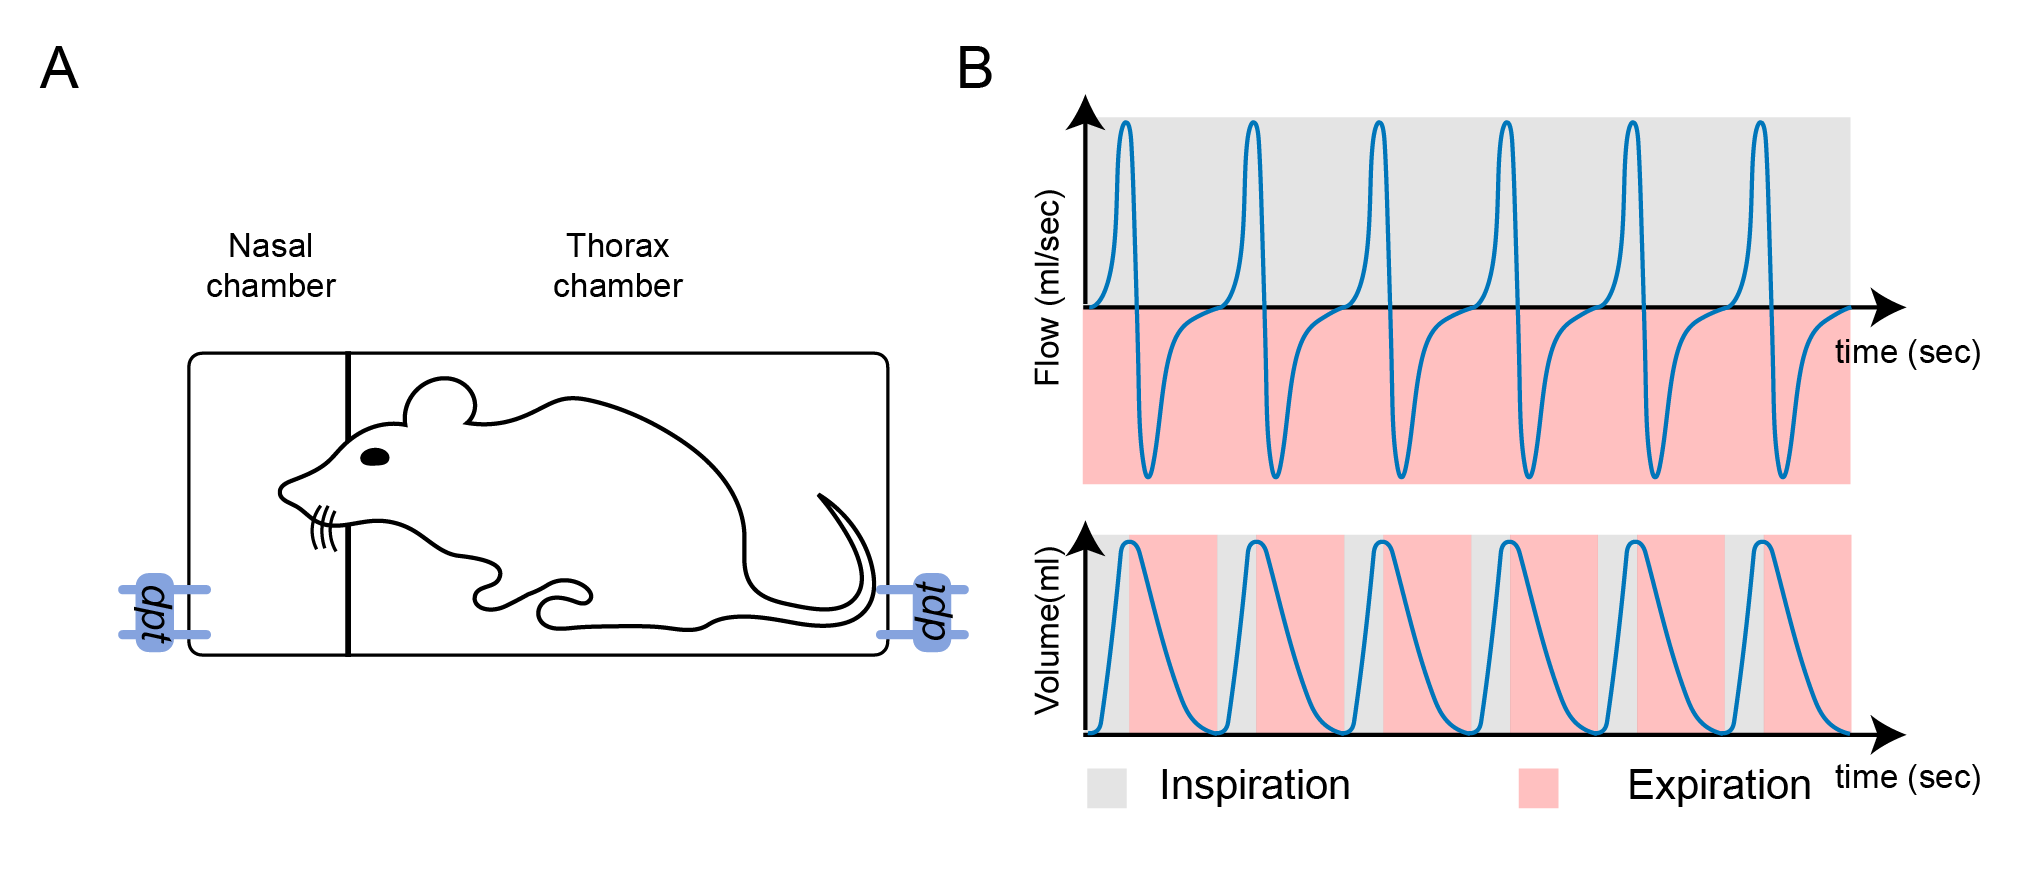
\includegraphics[width = \linewidth]{pictures/mice_exp.png}
  \caption{A: Illustration of a double-chamber plethysmograph. The term \textit{dpt} stands for differential 
  pressure transducer which measures the pressure in each compartment, the pressure then being converted to flow. 
  B: Nasal airflow (top) and lung volume (bottom). During inspiration, airflow is positive (grey) and during
  expiration, airflow is negative (pink).}
  \label{fig:mice_exp}
\end{figure}

\label{appendix:mouse_dataset}
Ventilation is a simple physiological function that ensures a vital supply of oxygen and the elimination of CO2. 
Acetylcholine (Ach) is a neurotransmitter that plays an important role in muscular activity, notably for breathing. 
Indeed, muscle contraction information passes from the brain to the muscle through the nervous system. Achs are located 
in synapses of the nervous system (central and peripheral) and skeletal muscles. They ensure the information transmission 
from nerve to nerve. However, the transmission cannot end without the hydrolysis of Ach by the enzyme Acetylcholinesterase 
(AchE), allowing nerves to return to their resting state. Inhibition of (AchE) with, for instance, nerve gas, pesticide, 
or drug intoxication leads to respiratory arrests. 

The dataset comes from the experiment \cite{nervo2019respiratory}, where they studied the consequences of partial 
deficits in AChE and AChE inhibition on mice respiration. AchE inhibition was induced with an 
irritant molecule called physostigmine (an AchE inhibitor). Mice nasal airflows were sampled at 
2000Hz with a Double Chamber plethysmograph \cite{hoymann2012lung}, as depicted in \Cref{fig:mice_exp}-A). The flow is expressed in 
$ml.s^{-1}$; it has a positive value during inspiration and a negative value expiration \Cref{fig:mice_exp}-B). 
Among the mice population, we selected 7 control mice (\textbf{wt}) and 7 ColQ mice (\textbf{colq}), which do not have 
AChE anchoring in muscles and some tissues. 
As described in \cite{nervo2019respiratory}, mice experiments were as follows:
\begin{enumerate}
  \item The mouse is placed in a DCP for 15 or 20 min to serve as an internal control.
  \item The mouse is removed from the DCP and injected with physostigmine.
  \item The mouse is placed back into the DCP, and its nasal flow is recorded for 35 or 40 min.
\end{enumerate}

Respiratory cycles were extracted following procedure \cite{germain2023unsupervised}. We removed 
respiratory cycles whose duration exceeds 1 second; the average respiratory cycle duration is 
300 ms. We randomly sampled 10 respiratory cycles per minute and mouse. It leads to a dataset of 
12,732 (time, genotype)-annotated respiratory cycles. 

\subsection{Shape-based UCR/UEA time series classification datasets}
\label{appendix:classification_dataset}
We selected 15 shape-based datasets (7 univariates and 8 multivariates) from the from the University of East Anglia (UEA) and the University of California Riverside (UCR) Time Series Classification Repository\footnote{https://timeseriesclassification.com} \cite{dau2019ucr,bagnall2018uea}. All datasets were downloaded with the python package aeon\footnote{https://www.aeon-toolkit.org/en/stable/}. Essential datasets information are summarized in \Cref{appendix:table:datasets} and further can be found in \cite{dau2019ucr,bagnall2018uea}.

\begin{table}[hbt!]
  \centering
  \caption{UCR/UEA shape-based time series datasets for classification.}
  \resizebox{\columnwidth}{!}{%
  \begin{tabular}{lllllll}
    \toprule
    & \textbf{Dataset} &  \textbf{Size} & \textbf{Lengh} & \textbf{Number of classes} & \textbf{Number of dimensions} & \textbf{Type} \\
    \midrule
    \multirow[c]{7}{*}{Univariate} &  ArrowHead & 211 & 251 & 3 & 1 & IMAGE \\
    & BME & 180 & 128 & 3 & 1 & SIMULATED \\
    & ECG200 & 200 & 96 & 2 & 1 & ECG \\
    & FacesUCR & 2250 & 131 & 14 & 1 & IMAGE \\
    & GunPoint & 200 & 150 & 2 & 1 & MOTION \\
    & PhalangesOutlinesCorrect & 2658 & 80 & 2 & 1 & IMAGE \\
    & Trace & 200 & 275 & 4 & 1 & SENSOR \\
    \cline{1-7}
    \multirow[c]{8}{*}{Multivariate}& ArticularyWordRecognition & 575 & 144 & 25 & 9 & SENSOR \\
    & Cricket & 180 & 1197 & 12 & 6 & MOTION \\
    & ERing & 60 & 65 & 6 & 4 & SENSOR \\
    & Handwriting & 1000 & 152 & 26 & 3 & MOTION \\
    & Libras & 360 & 45 & 15 & 2 & VIDEO \\ 
    & NATOPS & 360 & 51 & 6 & 24 & MOTION \\
    & RacketSports & 303 & 30 & 4 & 6 & SENSOR \\
    & UWaveGestureLibrary & 240 & 315 & 8 &3 & SENSOR \\
    \bottomrule
  \end{tabular}
  %
  }
  \label{appendix:table:datasets}
\end{table}

\section{Experiments}

\subsection{Identifiability experiments}
\label{appendix:identifiability}

\begin{figure}[t]
  \centering
  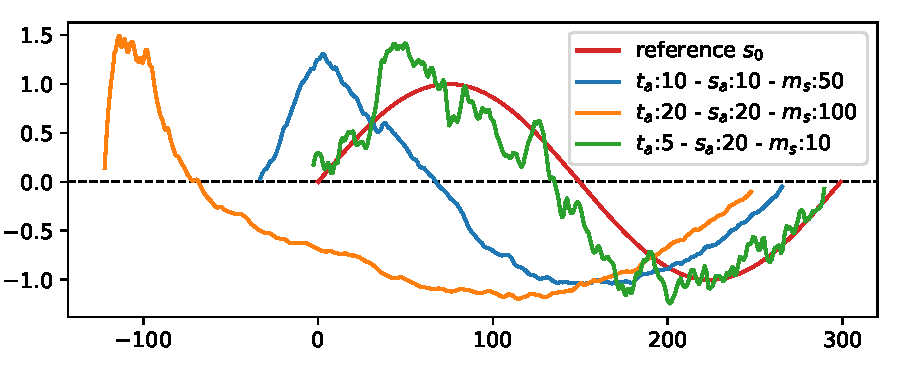
\includegraphics[width=0.5\linewidth]{pictures/samples.pdf}
  \vspace{-2.5em}
  \caption{Plots of $\varphi^{\{v_0(\mathbf{\alpha}^*,\msx)\}}.\msx$ for different values of $\mathbf{\alpha}^*$ according to its sampling parameter $t_a,s_a,m_s $, taking $\msx=\msg(s_0)$ with $s_0:k\in [300]\to \sin(2\pi k/300) $.}
  \label{fig:exemple_synthetic}
  \vspace{-1em}
\end{figure}

\begin{table}
  \caption{Values of $\scrl(\varphi^{\{v_0(\mathbf{\alpha}^*,\msx)\}}.\msx,\varphi^{\{\hat{v}_0\}}.\msx)$ as $\mathbf{\alpha}^*$ is sampled according to Gen(10,10,50) and $\hat{v}_0$ is estimated using $K_\msg$ with varying parameters $\sigma_{T,1},\sigma_x$.}
    \centering
       \begin{tabular}{lrrrrrrr}
       \toprule
       $\sigma_{T,0} \backslash \sigma_x$  & 1 & 10 & 50 & 100 & 200 & 300 \\
       \midrule
       0.1 & 2e+0 & 3e-4  & 1e-5&4e-6&7e-4&4e-3 \\
      1 & 4e-2 & 1e-4  & 1e-5&4e-6&7e-4 &4e-3  \\
       100 & 4e-2 & 2e-4  & 1e-5&4e-6&7e-4&4e-3  \\
       \bottomrule
       \end{tabular}
    \label{table:synthetic2}
    \vspace{-1em}
\end{table}



% \begin{subfigure}{0.7\linewidth}
%   \centering
%   \resizebox{\columnwidth}{!}{%
%      \begin{tabular}{lrrrr}
%      \toprule
%      $\sigma_{T,0} \backslash \sigma_x$  & 0.1 & 1 & 100 \\
%      \midrule
%      1 & 2e+0 & 4e-2 & 4e-2 \\
%      10 & 3e-4 & 1e-4  & 2e-4 \\
%      50 & 1e-5 & 1e-5  & 1e-5 \\
%      100 & 4e-6 & 4e-6 & 4e-6 \\
%      200 & 7e-4 & 7e-4 & 7e-4 \\
%      300 & 4e-3 & 4e-3 & 4e-3 \\
%      \bottomrule
%      \end{tabular}
%      %
%      }
%  \caption{Values of $\scrl(y^*,\varphi^{\{\hat{v}_0\}}.\msx)$ where $y^*$ is sampled according to Gen(10,10,50) and $\hat{v}_0$ is estimated using $K_\msg$ with varying parameters $\sigma_{T,1},\sigma_x$.}
% \end{subfigure}

provided that the hyperparameters and the reference graph are wisely selected, i.e., the parameter $v_0^*$ generating a deformation $\varphi^{\{v_0^*\}}$ of a time series graph $\msg$ can be estimated from the data $\msg,\varphi^{\{v_0^*\}}.\msg$ by solving the geodesic shooting problem \eqref{eq:relaxation}. 

First, we show the model identifiability when the kernel $K_G$ is well specified: the estimated parameter is a good approximation of the generating parameter when the generation and the estimation procedure use the same hyperparameters for the RKHS kernel $K_\msg$.
All the hyperparameter values for generation and estimation are given in \Cref{appendix:numerics_synthetic}.
We fix the initial control points as $\msx=\left(x_k=(k,\sin(2\pi k/300))\right)_{k\in[300]} $.
Given $m_{s}\in \Nset_{>0}$ and $t_{a},s_{a}>0$, we randomly generate initial momentums $\mathbf{\alpha}^*=(\alpha_k^*)_{k\in[\mathbf{n}_0]}$ with the following sampling, called Gen($m_s,t_a,s_a$):
For any $k\in[\mathbf{n}_0]$, $\mathbf{\alpha}_k'$ is sampled according to a Gaussian normal distribution $\mathcal{N}(0_{d+1},I_{d+1})$.
Then, $(\alpha_k')_{k\in[\mathbf{n}_0]}$ is regularized by a rolling average of size $m_{s}$, we get $\bar{\mathbf{\alpha}}'=(\bar{\alpha}_k')_{k\in[\mathbf{n}_0]}$.
Finally, we normalize $\bar{\mathbf{\alpha}}'$ to derive $\mathbf{\alpha}^*$ such that $|([\alpha_k^*]_t)_{k\in[\mathbf{n}_0]}|=t_{\text{amp}}$ and $|([\alpha_k^*]_s)_{k\in[\mathbf{n}_0]}|=s_{\text{amp}}$ for any $k\in[\mathbf{n}_0]$, denoting by $[\alpha_k^*]_t,[\alpha_k^*]_s$ the time and space coordinates of $\alpha_k^*$ respectively.
Note that the regularizing step $(\mathbf{\alpha}_k')_{k\in[\mathbf{n}_0]}\to \bar{\mathbf{\alpha}}' $ is necessary to obtain realistic deformations which take into account the regularity induced by the RKHS $\msv$.
%  uniformly on the set $\mss_M=\{ (\alpha_k)_{k\in[\mathbf{n}_0]}\in (\Rset^{d+1})^{\mathbf{n}_0}:\eqsp |\alpha_k|=M\}  $ with $M>0,\mathbf{n}_0\in \Nset_{>0}$,
%  then we regularize $\mathbf{\alpha}$ by convolving
%   with ... to get the generation parameter $\mathbf{\alpha}^*$.
Then, using $v_0(\mathbf{\alpha}^*,\msx)$ as defined in \eqref{eq:def_v0} with initial momentums $\mathbf{\alpha}^*$ and control points $\msx$, we apply the induced deformation $\varphi^{\{v_0\}} $ by \eqref{eq:integration} to $\msx$ and obtain $\varphi^{\{v_0\}}.\msx$.
Finally, we solve \eqref{eq:relaxation} to recover an estimation $\hat{\mathbf{\alpha}}$ of $\mathbf{\alpha}^*$ and report the average relative error (ARE) $|v_0(\hat{\mathbf{\alpha}},\msx)-v_0(\mathbf{\alpha}^*,\msx)|_\msv/|v_0(\mathbf{\alpha}^*,\msx)|_\msv$ on 50 repetitions.
This procedure is performed for any $m_{s},t_{a},s_{a}\in \{10,50,100\}\times \{5,10,15,20\}^2 $.
Mean, standard deviation, and maximum of the ARE on all these hyperparameters choices are respectively $\mathbf{0.10, 0.03, 0.17}$.
Therefore, the estimation procedure \eqref{eq:relaxation} offers a good approximation of the true parameter when the kernel $K_\msg$ is well specified.
We observe that the estimation is difficult when $t_a\ll s_a$ because the time series can be very noisy as illustrated in \Cref{fig:exemple_synthetic}: this impacts the Varifold loss which is sensitive to tangents.

Secondly, we demonstrate a weak identifiability when the kernel $K_\msg$ is misspecified: we can reconstruct the graph time series' after deformations even if the hyperparameters of $K_\msg$
are different during the generation and the estimation.
 The hyperparameters of $K_\msg$ during generation are $(c_0,c_1,\sigma_{T,0},\sigma_{T,1},\sigma_x)=(1,0.1,100,1,1)$ and we fix $\sigma_{T,1},c_0,c_1=(1,1,0.1) $ for $K_\msg$ during estimation.
 We aim to understand the impact of $\sigma_{T,1},\sigma_x$ on the reconstruction since they are encoding the smoothness of the transformation according to time and space.  

  For any choice of the hyperparameters $\sigma_{T,1},\sigma_x\in \{1,10,50,100,200,300 \}\times \{0.1,1,100\}$ related to $K_\msg$ in the estimation,
   we average $\scrl(\varphi^{\{v_0(\mathbf{\alpha}^*,\msx)\}}.\msx,\varphi^{\{\hat{v}_0\}}.\msx)$ on 50 repetitions when $\mathbf{\alpha}^*$ is sampled according to Gen$(10,10,50)$ and $\hat{v}_0=v_0(\hat{\alpha},\msx)$ denoting by $\hat{\alpha}$ the result of the minimization \eqref{eq:relaxation}.
We observe in \Cref{table:synthetic2} that the reconstruction is almost perfect except in the case when $\sigma_{t,0}=1$ during estimation, while $ \sigma_{t,0}=100$ during generation.
 Compared to $\sigma_{T,0}$, $\sigma_x$ has nearly no impact on the reconstruction.
 In \Cref{appendix:kernel_implementation}-\ref{appendix:kernel_TS_LDDMM}, we propose guidelines to drive future hyperparameters tuning and further discussions related to $\sigma_{T,1},c_0,c_1$. 


\subsection{Classification: Comparison with shape analysis methods}
\label{appendix:classification_shape_analysis}

In this section, we compare classification performances of TS-LDDMM with other state-of-the-art methods coming from shape analysis on 15 shape-based datasets of time-series.

\paragraph{Methods} We compare TS-LDDMM with a method from function~\cite{wu2024shape}

\paragraph{Protocole}

\begin{table}[hbt!]
  \centering
  \resizebox{\columnwidth}{!}{%
  \begin{tabular}{llrrrr}
    \toprule
     & \textbf{Dataset} & \textbf{Shape-FPCA (2024)} & \textbf{TCLR (2024)} & \textbf{LDDMM (2008)} & \textbf{TS-LDDMM (ours)} \\
    \midrule
    \multirow[c]{7}{*}{Univariate} & ArrowHead & 0.18 & 0.75 & \underline{0.84} & \textbf{0.91} \\
     & BME & 0.16 & \underline{1.00} & 0.82 & \textbf{1.00} \\
     & ECG200 & 0.40 & 0.67 & \textbf{0.81} & \underline{0.79} \\
     & FacesUCR & 0.08 & \underline{0.73} & 0.69 & \textbf{0.86} \\
     & GunPoint & 0.93 & \underline{0.97} & 0.83 & \textbf{1.00} \\
     & PhalangesOutlinesCorrect & 0.39 & \textbf{0.63} & \underline{0.53} & 0.52 \\
     & Trace & 0.55 & \underline{1.00} & 0.46 & \textbf{1.00} \\
    \cline{1-6}
    \multirow[c]{8}{*}{Multivariate} & ArticularyWordRecognition & -- & -- & \underline{0.98} & \textbf{1.00} \\
     & Cricket & -- & -- & \underline{0.77} & \textbf{0.93} \\
     & ERing & -- & -- & \underline{0.95} & \textbf{0.98} \\
     & Handwriting & -- & -- & \underline{0.22} & \textbf{0.44} \\
     & Libras & -- & -- & \underline{0.56} & \textbf{0.60} \\
     & NATOPS & -- & -- & \underline{0.82} & \textbf{0.82} \\
     & RacketSports & -- & -- & \textbf{0.83} & \underline{0.79} \\
     & UWaveGestureLibrary & -- & -- & \underline{0.72} & \textbf{0.81} \\
    \bottomrule
    \end{tabular}
    %
  }
    
\end{table}


\section{Robustness to missing data}

\begin{table}[hbt!]
  \centering
  \begin{tabular}{lcccc}
    \toprule
    \multirow[c]{2}{*}{\textbf{Methods}} & \multicolumn{4}{c}{\textbf{Test F1-score}} \\
    \cline{2-5}
     &  \textbf{Regular} & \textbf{30 \% dropped} &  \textbf{50 \% dropped} & \textbf{70 \% dropped} \\
    \midrule
    RNN (1999) & $0.64 \pm 0.21$ & $0.53 \pm 0.23$ & $0.48 \pm 0.21$ & $0.44 \pm 0.21$ \\
    LSTM (1997) & $0.61 \pm 0.29$ & $0.57 \pm 0.29$ & $0.53 \pm 0.25$ & $0.51 \pm 0.29$ \\
    GRU (2014) & $0.71 \pm 0.26$ & $0.68 \pm 0.28$ & $0.66 \pm 0.28$ & $\underline{0.59 \pm 0.28}$ \\
    MTAN (2021) & $0.59 \pm 0.28$ & $0.58 \pm 0.28$ & $0.54 \pm 0.29$ & $0.51 \pm 0.28$ \\
    MIAM (2022) & $0.48 \pm 0.35$ & $0.42 \pm 0.33$ & $0.47 \pm 0.31$ & $0.35 \pm 0.31$ \\
    ODE-LSTM (2020) & $0.63 \pm 0.24$ & $0.57 \pm 0.25$ & $0.51 \pm 0.24$ & $0.45 \pm 0.23$ \\
    Neural SDE (2019) & $0.48 \pm 0.28$ & $0.47 \pm 0.26$ & $0.45 \pm 0.27$ & $0.45 \pm 0.25$ \\
    Neural LNSDE (2024) & $0.7 \pm 0.27$ & $0.68 \pm 0.29$ & $\underline{0.67 \pm 0.25}$ & $\mathbf{0.66 \pm 0.23}$ \\
    LDDMM (2008) & $\underline{0.72 \pm 0.2}$ & $\underline{0.7 \pm 0.21}$ & $0.57 \pm 0.25$ & $0.4 \pm 0.25$ \\
    %\cline{1-5}
    TS-LDDMM (ours) & $\mathbf{0.83 \pm 0.18}$ & $\mathbf{0.8 \pm 0.18}$ & $\mathbf{0.7 \pm 0.26}$ & $0.51 \pm 0.27$ \\
    \bottomrule
  \end{tabular}  
\end{table}




    
%  [11:35, 31/01/2024] Thibaut Germain: avant/après :
%  [11:35, 31/01/2024] Thibaut Germain: Kv = VFTSGaussKernel(1,0.1,150,1,1)
%  Kl = TSGaussGaussKernel(5,1,5,0.6)
%  dataloss = VarifoldLoss(Kl)
%  schedule = warmup_cosine_decay_schedule(0,0.3,80,800,0)
%  [11:35, 31/01/2024] Thibaut Germain: avant :
%  [11:35, 31/01/2024] Thibaut Germain: Kv = VFTSGaussKernel(1,0.1,100,1,1)
%  Kl = TSGaussGaussKernel(2,1,2,0.6)
%  dataloss = VarifoldLoss(Kl)
%  schedule = warmup_cosine_decay_schedule(0,0.3,40,400,0)
% Let $s$ be a time series and $\msg(\tilde{s}) = (g_i)_{i \in [n]}$ be its discretized graph.
%  The graph $\msg(s)$ can be approximated as 
% the union of piecewise linear segments between time-consecutive samples, 
% and we associate to the approximated graph the oriented varifold:

% \begin{equation}
%   \mu_{\msg(\tilde{s})} : w \in \msw \mapsto \sum_{i=1}^{n-1} l_i\delta_{(c_i,\overrightarrow{v_i})}(w)
% \end{equation}
% where $\msw$ is a set of real valued test functions defined on $\Rset^{d+1} \times \mathbb{S}^d$, 
% $\delta_{(c_i,\overrightarrow{v_i})}(w) = w(c_i,\overrightarrow{v_i})$ is a Dirac delta function, 
% $c_i = (g_i + g_{i+1})/2$ (resp. $v_i = \| g_{i+1}-g_{i}\|$) is the center (resp. length) of the $i^{th}$ segment, 
% and $\overrightarrow{v_i} = (g_{i+1}-g_{i})/l_i$ is the unit norm vector of direction $\overrightarrow{g_i g_{i+1}}$.

% Assuming that the test functions' space $\msw$ is the RKHS associated with a $C^1$ positive definite kernel $k$ 
% that verifies \citep[Proposition 2 \& 4]{kaltenmark2017general}, the oriented varifold belongs to the dual space $\msw^*$. Additionally, 
% we can define a distance $d_{\msw^*}$ between signals' graph sample sets, which, thanks to the kernel reproducing property,
% has an explicit formulation: 


% \section{Continuous normalizing flows}
% %Modeling Continuous Stochastic Processes with Dynamic Normalizing Flows time series generative
% CONTUNYIYS NORMALIZING FLOW bofbof
% Here, we present the framework of Continuous Normalizing Flows (CNF) and show how LDDMM can be seen as a particular case.
% \cite{salman2018deep} was already inspired from the work of shape analysis to present deep diffeomorphic normalizing flows.
% Discussion with Alain :
% Given a time-dependant vector field $v:[0,1]\times \Rset^{d'} \to \Rset^{d'} $, the integration of this vector field gives a flow $ \phi:[0,1]\times \Rset^{d'} \to \Rset^{d'}$, defined via the ordinary differential equation (ODE),
% \begin{equation}
%   \frac{\dd }{\dd \tau}\phi_\tau(x)=v(\tau,\phi_\tau(x)), \phi_0(x)=x \eqsp.
%  \end{equation}
% In \cite{chen2018neural}, they introduce Continous Normalizing flows for generative modeling.
%  By modeling $v=f_\theta$ is a neural networks and choosing a prior $X_0\sim\rho_0$ on the inital value, the law of $\phi_1(X_0)$ has the pullback density $\phi_1\# \rho_0$ and the parameter $\theta$ is optimized to maximize the log-likelihood of a given dataset $(y_i)_{i\in[N]}\in (\Rset^{d'})^N$ which is assumed to follow the law of $\phi_1(X_0)$.
% Instead of modeling the law of the end point $\phi_1(X_0) $, we can try to model the law of the whole path $(\phi_\tau(X_0))_{\tau\in[0,1]} $ having a density $p:[0,1]\times \Rset^d\to \Rset_{>0}$ such that $p_1=q, p_0=\rho_0$ where $q$ is the empirical distribution in the dataset, as proposed in \cite{lipman2022flow}.
% In so doing, the problem is ill-posed since $p_t$ can be whatever as soon as $0<t<1$, that is why we try to constraint the learned velocity field $v=f_\theta$ such that the path law $p$ is tractable.
% One way of doing it is to look for geodesics \eqref{eq:geodesics_original} as proposed in LDDMM, it corresponds to the case where $q=\sum_{i=1}^N \delta_{y_i}/N$ and $\rho_0=\sum_{i=1}^N \delta_{x_i}/N$ are empirical distribution and $y_i=\phi^v_1(x_i) $ for a given velocity field $v$.

% The goal is to target $\nu\in \mathcal{P}(\rmC^0([0,1]\times \Rset^d, \Rset^d)) $ by generating randomness on a initial value $x \sim \delta_x$
%  and by integrating a velocity field $v_\theta \in \msw \subset \rmC^0([0,1]\times \Rset^d, \Rset^d)$: 
%  \begin{equation}
%   \frac{\dd h}{\dd \tau}=v_\theta(\tau,h(\tau,x)), h(0,x)=x \eqsp,
%  \end{equation}
%  denoting by $\mu$ the law of $(h(\tau,x))_{\tau \in [0,1]}$. 

%%%%%%%%%%%%%%%%%%%%%%%%%%%%%%%%%%%%%%%%%%%%%%%%%%%%%%%%%%%%%%%%%%%%%%%%%%%%%%%
%%%%%%%%%%%%%%%%%%%%%%%%%%%%%%%%%%%%%%%%%%%%%%%%%%%%%%%%%%%%%%%%%%%%%%%%%%%%%%%


% \subsection{TTS}
% To circumvant this issue, we propose two methods :
%       \begin{enumerate}
%         \item \label{enum:first_method} [Time And Space (TAS)] Using a specific form of the RKHS's kernel in LDDMM, to stick to the classical shape analysis framework.
%         \item \label{enum:second_method} [Time Then Space (TTS)] Tackling the time axis and space axis separetely in the transformation.
%          This distangles time and space variability in the patterns, increasing the interpretability of the representation.
%           Although the related optimization is more complex than method \ref{enum:first_method}, the results is more robust to the choice of hyper-parameter related to the RKHS's kernel.
%       \end{enumerate}
%        In the following, we present both methods to highlights their pro and cons.


% As described in \Cref{section:optimization}, the method (TAS) learns $\Pi_{\gamma,f}$ directly, while (TTS) find the temporal reparametrisation $\Phi_f$ then the space transformation $\Psi_\gamma$.
%     % If we define a diffeomorpshim $\Phi_\gamma$ as $(\gamma,\Id_d) $, we have $\Phi_\gamma.G(s) =G(s).\gamma^{-1}$.
%     %  To increase the variability, we allow some deformations on the graph of the time series after being reparametrized in time, which allow us to recover every possible time seriess.
%     % Remark that, $G(\mathbf{s}_0\circ \psi^{-1})=\{(t,\mathbf{s}_0\circ \psi^{-1}(t)), t\in \msj \}= \{(\psi(t),\mathbf{s}_0(t)) ,\eqsp t\in \msi \}  $.
%     % [The action of the diffeomorpshim group 
%     % \begin{align}
%     %     &\mcd_*=\mcd(\Rset,\Rset)\times \{\phi\in \mcd(\Rset^{d+1},\Rset^{d+1}): \\
%     %     &\phi(t,x)=(t,f(t,x)),
%     %      (t,x)\in \Rset \times \Rset^{d}, f \in C^0(\Rset^{d+1}, \Rset^d) \} 
%     % \end{align}
%     % on the space of time series graph $\{G^{(a,b)}(s), s\in C^0((a,b), \Rset), (a,b)\in \Rset_+^2, a<b  \}$
%     % is homogene.]
%      %In the next section we define a metric and a norm on this space in order to find a representation $(\phi,\psi)$ with a minimal norm, and we show in (...) how to recover a proxy.
%      \paragraph{The representation as the solution of an optimization}
%      By \Cref{theorem:representation}, for any $\mathbf{s}_0\in C^0(\msi,\Rset^d)$, we can find $ F=(\gamma_j,f_j)_{j\in[N]}$ such that $\msg(s^j)=\Pi_{\gamma_j,f_j}.\msg(\mathbf{s}_0)$ for any $j\in[N]$.
%      However, to get a meaningfull representation and to tackle the unicity problem, we should optimize the choice of $\mathbf{s}_0 $ and $F$, formally speaking, denoting by $R(\cdot) $ a regularization norm on $\mcd(\Rset^{d+1})$ and $L$ a loss on sets which will be specify later, we aim to solve
%      \begin{equation}
%       \label{eq:minimization}
%       \underset{\mathbf{s_0},(\gamma_j,f_j)_{j\in[N]}}{ \argmin} \sum_{j=1}^N \lambda R(\Pi_{\gamma_j,f_j})+ L(\msg(s^j),\Pi_{\gamma_j,f_j}.\msg(\mathbf{s}_0)) \eqsp ,
%     \end{equation} 
%     where $\lambda>0$ is a penalization factor related to $L$ to relax the condition $\msg(s^j)=\Pi_{\gamma_j,f_j}.\msg(\mathbf{s}_0)$.

%     In practice, as already proposed in shape analysis, we perform an alternative minimization between $\mathbf{s_0}$ and $(\gamma_j,f_j)_j$.
%     The optimization on $(\gamma_j,f_j)_j$ is parrallelisable, for each couple $(\mathbf{s}_0,s^j)$, we should learn diffemorphisms of minimal norm satisfying a condition. 
%     To this end, we adapt the geodesic shooting method using LDDMM presented in \cite{durrleman2013sparse} to our special case.
%       Before to describe how to optimize the whole in \Cref{section:optimization}, we introduce LDDMM in the next section to specify the norm on diffemorphisms.

% \paragraph{Kernel choices}
% As depicted on figure (mettre ref), we can not use any kernel $K$ to apply the previous methodology to learn deformations on time series' graphs.

% In the following, we expose two choice of RKHS's kernel which answers this issue : (TAS) and (TTS).
%  We rely on the Gaussian kernel, denoting by $K_\sigma^{(a)}(x,y)=\exp(-|x-y|^2/\sigma)$ for any $(x,y)\in (\Rset^a)^2$, $a\in \Nset$ and $\sigma>0$.
% To apply (TAS) in LDDMM with $d'=d+1$, we use the following anisotropic Gaussian kernel  :
% \begin{align}
%   \label{eq:kernel_TAS}
%   &K_{\text{TAS}}((t,x),(t',x'))=\begin{pmatrix}
%     c_0K & 0 \\
%     0 & c_1 D 
%     \end{pmatrix} \eqsp , \\
%     &D=K_{\sigma_{T,1}}^{(1)}(t,t')K_{\sigma_x}^{(d)}(x,x') \Idd\eqsp,K=K_{\sigma_{T,0}}^{(1)}(t,t') \eqsp,
% \end{align}
% parametrized by the widths $\sigma_{T,0},\sigma_{T,1},\sigma_x>0$ and the constants $c_0,c_1>0$.
%  If we use this kernel, by considering \eqref{eq:specific_form}, we remark that the first coordinate of the velocity field $v_\tau$ only depends on the time variable $t$.
%   It implies that the final deformation will have the form $\phi^v=(\gamma,f) $ with  $f\in C^1(\Rset^{d+1},\Rset^d) $, and $\gamma\in \mcd(\Rset)$
%   since the first coordinate follows a LDDMM-ODE \eqref{eq:LDDMM_dynamic}.


% To apply (TTS), we use LDDMM on the time axis with $d'=1$ by taking $K_{\text{TTS}}^{\text{time}}=K_{\sigma_{T,0}}^{(1)}$, then on the space axis with $d'=d$ by choosing
% $K_{\text{TTS}}^{\text{space}}=K_{\sigma_{T,1}}^{(1)}\times K_{\sigma_x}^{(d)} $ where the widths are the same than in \eqref{eq:kernel_TAS}. The alternate optimization will be more detailed in \Cref{section:optimization}.



% This document was modified from the file originally made available by
% Pat Langley and Andrea Danyluk for ICML-2K. This version was created
% by Iain Murray in 2018, and modified by Alexandre Bouchard in
% 2019 and 2021 and by Csaba Szepesvari, Gang Niu and Sivan Sabato in 2022.
% Modified again in 2023 by Sivan Sabato and Jonathan Scarlett.
% Previous contributors include Dan Roy, Lise Getoor and Tobias
% Scheffer, which was slightly modified from the 2010 version by
% Thorsten Joachims & Johannes Fuernkranz, slightly modified from the
% 2009 version by Kiri Wagstaff and Sam Roweis's 2008 version, which is
% slightly modified from Prasad Tadepalli's 2007 version which is a
% lightly changed version of the previous year's version by Andrew
% Moore, which was in turn edited from those of Kristian Kersting and
% Codrina Lauth. Alex Smola contributed to the algorithmic style files.
